\documentclass[12pt]{standalone}

\RequirePackage{times}
\RequirePackage{amsmath}
\RequirePackage{amssymb}
\RequirePackage[T1]{fontenc}

\usepackage{tikz}
\usepackage{xcolor}
\usepackage{pgfplots}
\pgfplotsset{compat=1.16}

\definecolor{red}{HTML}{972e21}
\definecolor{yellow}{HTML}{ebb83f}
\definecolor{blue}{HTML}{7999db}

\begin{document}
	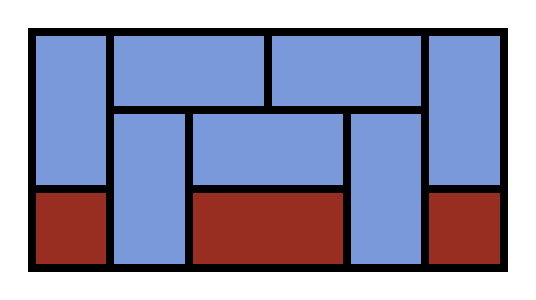
\begin{tikzpicture}[line width=0.1cm]
		\draw[fill=red] (0,0) rectangle(1,1);
		\draw[fill=red] (2,0) rectangle(4,1);
		\draw[fill=red] (5,0) rectangle(6,1);
		
		\draw[fill=blue] (0,1) rectangle(1,3);
		\draw[fill=blue] (1,0) rectangle(2,2);
		\draw[fill=blue] (2,1) rectangle(4,2);
		\draw[fill=blue] (4,0) rectangle(5,2);
		\draw[fill=blue] (5,1) rectangle(6,3);
		\draw[fill=blue] (1,2) rectangle(3,3);
		\draw[fill=blue] (3,2) rectangle(5,3);
	\end{tikzpicture}
\end{document}